\section{More about Event-B}

\subsection{Decomposition and Composition}

Decomposition and composition are two related approaches, that we use to partition a system, to allow us to work on smaller, manageable sub-models. Figure~\ref{fig:decomp2} illustrates the shared-event decomposition approach~\cite{decomp2010c} which we make use of in our code generation approach. An alternative shared-variable approach is described in~\cite{AbrialH07}. In the shared-event decomposition approach the system is partitioned so that each variable is allocated to a single machine. In the figure, the variables of machine $m$ are partitioned into the sets $v1$ and $v2$ and decomposed into $m_a$ and $m_b$ respectively. The events ....
 %
\begin{figure}
\centering
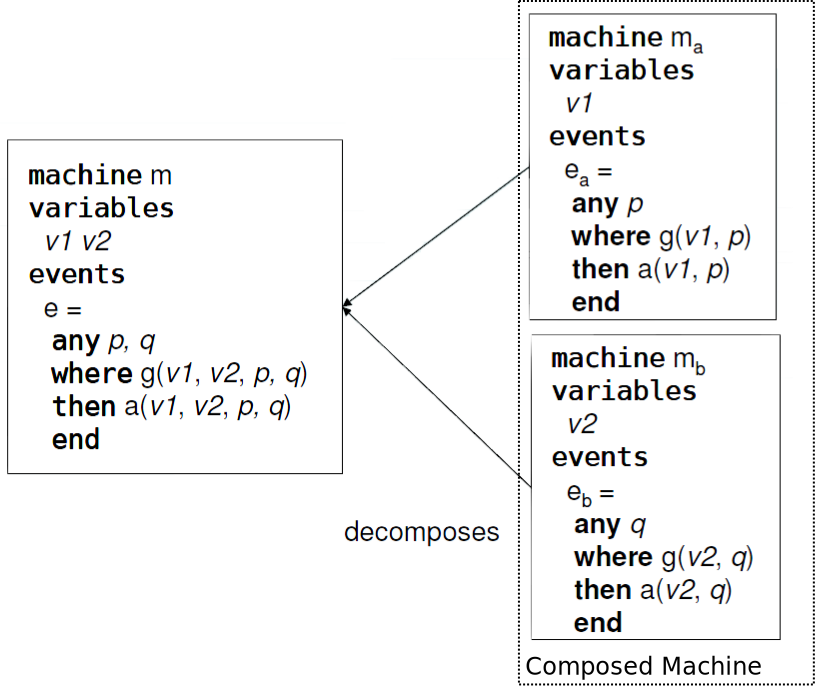
\includegraphics[width=0.5\textwidth]{graphics/Decomp2.png}
\caption{Decomposition}
\label{fig:decomp2}
\end{figure}





\subsection{Theories}

\subsection{ProB}
